\documentclass[10pt,a4paper,twocolumn]{article}

\usepackage[margin=1.8cm,top=1.6cm,bottom=1.6cm]{geometry}
\usepackage{booktabs}
\usepackage{tabularx}
\usepackage{graphicx}
\usepackage[table]{xcolor}
\usepackage{pgfplots}
\usepackage{pgfplotstable}
\usepackage{tikz}
\usepackage{enumitem}
\usepackage{microtype}
\usepackage{titlesec}
\usepackage[hidelinks]{hyperref}
\usepackage{caption}

\pgfplotsset{compat=1.18}

% Compact section spacing
\titlespacing*{\section}{0pt}{6pt}{3pt}
\titlespacing*{\subsection}{0pt}{4pt}{2pt}
\titleformat{\section}{\normalsize\bfseries}{\thesection.}{0.4em}{}
\titleformat{\subsection}{\small\bfseries}{\thesubsection}{0.4em}{}

\setlength{\parskip}{2pt}
\setlength{\parindent}{0pt}
\setlist{nosep,leftmargin=1.2em}

\definecolor{xcorr}{HTML}{3498DB}
\definecolor{outlier}{HTML}{2ECC71}
\definecolor{infill}{HTML}{9B59B6}
\definecolor{pccolor}{HTML}{C0392B}
\definecolor{oldpc}{HTML}{E6B0AA}
\definecolor{lightgray}{HTML}{F5F5F5}

\captionsetup{font=small,labelfont=bf,skip=4pt}

\begin{document}

\begin{center}
{\Large\bfseries PIV Pipeline Profiling Report}\\[3pt]
{\small 4-pass multi-grid (128\,$\to$\,64\,$\to$\,32\,$\to$\,16), 50\% overlap, Gaussian window, gauss6 peak finder}\\[2pt]
{\small\color{gray} 2026-02-26 \quad|\quad 4 threads \quad|\quad 12 pairs per batch \quad|\quad 3 iterations averaged \quad|\quad Windows}
\end{center}

\vspace{-2pt}
\rule{\columnwidth}{0.4pt}

\section{Key Finding}

The pipeline processes 4\,MP images at \textbf{0.17\,s/pair} across all 4 passes with 4 threads---a \textbf{1.8$\times$ overall speedup} over the previous \texttt{cv2.remap}-based pipeline (0.31\,s/pair). The fused C kernel (\texttt{libfusedwarp}) replaced Python mesh construction + \texttt{cv2.remap} image warping with a single OpenMP pass that upsamples the predictor and warps both images using bicubic interpolation (Keys $a$\,=\,$-$0.75).

The pipeline is now \textbf{xcorr-bound} at 4\,MP: \texttt{bulkxcorr2d} accounts for \textbf{43\%} of pass~4 runtime, while the predictor-corrector (fused warp) accounts for only 28\%. Previously, it was warp-bound at 54\%.

\section{Before vs After: Fused Warp C Kernel}

\begin{center}
\small
\begin{tabular}{@{}lrrr@{}}
\toprule
\textbf{Metric (4\,MP)} & \textbf{Before} & \textbf{After} & \textbf{Speedup} \\
\midrule
Grand total (s/pair) & 0.31 & 0.17 & 1.8$\times$ \\
Pass~4 total (s/pair) & 0.120 & 0.075 & 1.6$\times$ \\
\rowcolor{lightgray}
Pass~4 pred-corr (s/pair) & 0.065 & 0.021 & 3.1$\times$ \\
\quad mesh + cv2.remap warp & 0.043 & --- & \\
\quad dense pred remap & 0.021 & --- & \\
\quad fused\_warp (C kernel) & --- & 0.020 & \\
Pass~4 xcorr (s/pair) & 0.031 & 0.032 & --- \\
\midrule
Pass~4 pred-corr share & 54\% & 28\% & \\
Pass~4 xcorr share & 26\% & 43\% & \\
\bottomrule
\end{tabular}
\captionof{table}{Before/after comparison (4\,MP, biharmonic infilling, 4 threads). The fused C kernel eliminated the Python mesh construction and cv2.remap image warp, consolidating predictor upsampling + symmetric warp + bicubic interpolation into a single OpenMP loop.}
\end{center}

\section{Cost Breakdown: Before vs After}

\begin{center}
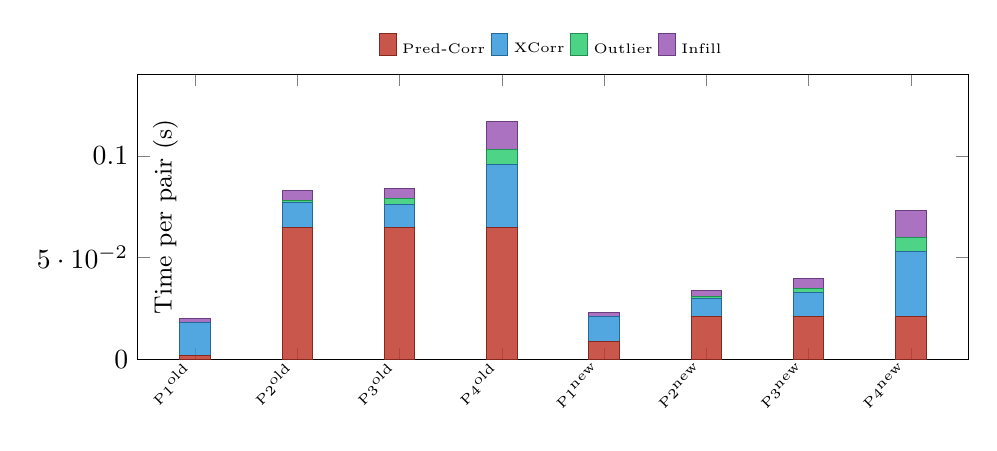
\begin{tikzpicture}
\begin{axis}[
    ybar stacked,
    bar width=11pt,
    width=\columnwidth,
    height=5.2cm,
    ymin=0, ymax=0.14,
    ylabel={\small Time per pair (s)},
    ylabel style={at={(axis description cs:0.06,0.5)}},
    symbolic x coords={P1\textsuperscript{old}, P2\textsuperscript{old}, P3\textsuperscript{old}, P4\textsuperscript{old}, P1\textsuperscript{new}, P2\textsuperscript{new}, P3\textsuperscript{new}, P4\textsuperscript{new}},
    xtick=data,
    x tick label style={font=\tiny, rotate=45, anchor=east},
    legend style={at={(0.5,1.02)}, anchor=south, legend columns=4, font=\tiny, draw=none},
    every axis plot/.append style={fill opacity=0.85},
    enlarge x limits=0.08,
    extra x ticks={},
    xticklabel style={
        /pgf/number format/.cd,
    },
]
% pred-corr
\addplot[fill=pccolor,draw=pccolor!70!black] coordinates {
    (P1\textsuperscript{old},0.002) (P2\textsuperscript{old},0.065) (P3\textsuperscript{old},0.065) (P4\textsuperscript{old},0.065)
    (P1\textsuperscript{new},0.009) (P2\textsuperscript{new},0.021) (P3\textsuperscript{new},0.021) (P4\textsuperscript{new},0.021)};
% xcorr
\addplot[fill=xcorr,draw=xcorr!70!black] coordinates {
    (P1\textsuperscript{old},0.016) (P2\textsuperscript{old},0.012) (P3\textsuperscript{old},0.011) (P4\textsuperscript{old},0.031)
    (P1\textsuperscript{new},0.012) (P2\textsuperscript{new},0.009) (P3\textsuperscript{new},0.012) (P4\textsuperscript{new},0.032)};
% outlier
\addplot[fill=outlier,draw=outlier!70!black] coordinates {
    (P1\textsuperscript{old},0.000) (P2\textsuperscript{old},0.001) (P3\textsuperscript{old},0.003) (P4\textsuperscript{old},0.007)
    (P1\textsuperscript{new},0.000) (P2\textsuperscript{new},0.001) (P3\textsuperscript{new},0.002) (P4\textsuperscript{new},0.007)};
% infill
\addplot[fill=infill,draw=infill!70!black] coordinates {
    (P1\textsuperscript{old},0.002) (P2\textsuperscript{old},0.005) (P3\textsuperscript{old},0.005) (P4\textsuperscript{old},0.014)
    (P1\textsuperscript{new},0.002) (P2\textsuperscript{new},0.003) (P3\textsuperscript{new},0.005) (P4\textsuperscript{new},0.013)};
\legend{Pred-Corr, XCorr, Outlier, Infill}
\end{axis}
\end{tikzpicture}
\captionof{figure}{Per-pair time by pass, before (left group) and after (right group) the fused warp C kernel. The predictor-corrector (red) dropped from 0.065\,s to 0.021\,s per pair on passes~2--4---a 3.1$\times$ reduction. XCorr and outlier/infill costs are unchanged.}
\end{center}

\section{Pass~4 Breakdown (Bottleneck Pass)}

\begin{center}
\small
\begin{tabular}{@{}lrr@{}}
\toprule
\textbf{Component} & \textbf{s/pair} & \textbf{\%} \\
\midrule
\texttt{fused\_warp} (C kernel) & 0.020 & 27 \\
\texttt{predictor\_remap}       & $<$0.001 & $<$1 \\
\rowcolor{lightgray}
\textit{Pred-Corr total}        & \textit{0.021} & \textit{28} \\
\texttt{bulkxcorr2d}            & 0.032 & 43 \\
\texttt{outlier\_det}           & 0.007 & 9 \\
\texttt{infilling}              & 0.013 & 17 \\
\midrule
\textbf{Pass total}              & \textbf{0.075} & \\
\bottomrule
\end{tabular}
\captionof{table}{Pass~4 per-pair breakdown (16$\times$16 windows, biharmonic infilling, 4\,MP). The fused C kernel replaced both \texttt{mesh\_and\_warp} (0.043\,s) and \texttt{dense\_pred\_remap} (0.021\,s) from the old pipeline with a single 0.020\,s call.}
\end{center}

\section{Predictor-Corrector: Fused Warp Internals}

The fused warp C kernel performs three operations in a single OpenMP-parallel loop over $(N \times H)$ rows:

\begin{enumerate}[leftmargin=1.4em]
\item \textbf{Predictor upsample:} Bicubic interpolation from the coarse window-center predictor grid to full pixel resolution.
\item \textbf{Symmetric coordinate maps:} $\mathbf{x}_A = \mathbf{x} - \tfrac{1}{2}\mathbf{d}$, $\mathbf{x}_B = \mathbf{x} + \tfrac{1}{2}\mathbf{d}$ for each pixel.
\item \textbf{Image interpolation:} Bicubic (Keys $a=-0.75$, 4$\times$4 stencil) or Lanczos-3 (6$\times$6 stencil, LUT-accelerated) sampling of both images.
\end{enumerate}

\begin{center}
\small
\begin{tabular}{@{}lrrrr@{}}
\toprule
\textbf{Sub-component} & \textbf{P1} & \textbf{P2} & \textbf{P3} & \textbf{P4} \\
\midrule
fused\_warp (C kernel)   & (skip) & 0.021 & 0.021 & 0.020 \\
gaussian\_smooth          & --- & $<$0.001 & $<$0.001 & $<$0.001 \\
predictor\_remap          & --- & $<$0.001 & $<$0.001 & $<$0.001 \\
\midrule
\textbf{Total}            & 0.009 & 0.021 & 0.021 & 0.021 \\
\bottomrule
\end{tabular}
\captionof{table}{Predictor-corrector per-pair sub-timings (seconds, 4\,MP). The fused warp is $O(\text{pixels})$---constant across passes~2--4 regardless of window count. Gaussian smoothing and predictor remap (window-center grid) are negligible.}
\end{center}

\noindent Eliminating intermediate allocations was key: the old pipeline allocated a $(N, H, W, 2)$ float32 coordinate mesh per image pair before calling \texttt{cv2.remap}. The fused kernel computes coordinates on-the-fly, never materialising the mesh.

\section{Scaling Behaviour: Per-Pass Cost}

\begin{center}
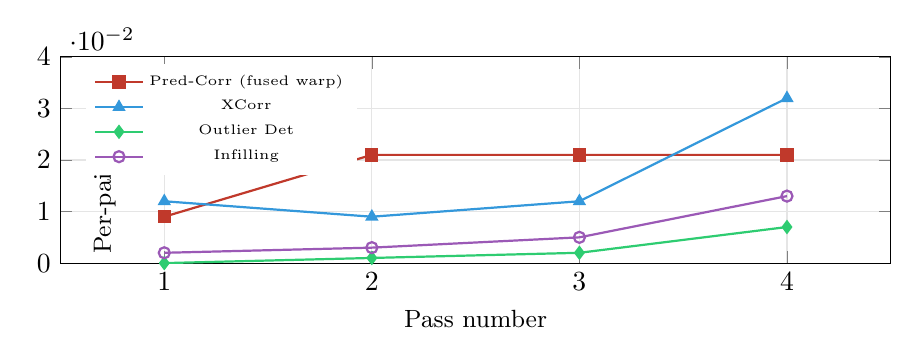
\begin{tikzpicture}
\begin{axis}[
    width=\columnwidth,
    height=4.2cm,
    xlabel={\small Pass number},
    ylabel={\small Per-pair time (s)},
    ylabel style={at={(axis description cs:0.08,0.5)}},
    xmin=0.5, xmax=4.5,
    ymin=0, ymax=0.04,
    xtick={1,2,3,4},
    legend style={at={(0.03,0.97)}, anchor=north west, font=\tiny, draw=none},
    grid=major,
    grid style={gray!20},
    every axis plot/.append style={thick},
]
\addplot[color=pccolor, mark=square*, mark size=2] coordinates {(1,0.009) (2,0.021) (3,0.021) (4,0.021)};
\addlegendentry{Pred-Corr (fused warp)}
\addplot[color=xcorr, mark=triangle*, mark size=2] coordinates {(1,0.012) (2,0.009) (3,0.012) (4,0.032)};
\addlegendentry{XCorr}
\addplot[color=outlier, mark=diamond*, mark size=2] coordinates {(1,0.000) (2,0.001) (3,0.002) (4,0.007)};
\addlegendentry{Outlier Det}
\addplot[color=infill, mark=o, mark size=2] coordinates {(1,0.002) (2,0.003) (3,0.005) (4,0.013)};
\addlegendentry{Infilling}
\end{axis}
\end{tikzpicture}
\captionof{figure}{Per-pair component cost by pass (4\,MP, 4 threads). The fused warp (red) is constant at ${\sim}$0.021\,s for passes~2--4---it scales with pixels, not windows. XCorr and infilling grow with window count, dominating pass~4.}
\end{center}

\section{Why It's This Fast: C + OpenMP}

The fused warp kernel uses OpenMP \texttt{schedule(static)} parallelism over $(N \times H)$ rows. Unlike the previous \texttt{ThreadPoolExecutor}-based parallelism (which relied on \texttt{cv2.remap} releasing the GIL), the C kernel runs entirely outside Python with no GIL contention.

\subsection{Batch Scaling (4\,MP, Pass~4)}

The C kernel's batch interface (\texttt{fused\_symmetric\_warp\_batch}) processes all $N$ images in a single call, amortising OpenMP thread-pool overhead:

\begin{center}
\small
\begin{tabular}{@{}lrr@{}}
\toprule
\textbf{Batch size} & \textbf{fused\_warp (ms/pair)} & \textbf{Overhead} \\
\midrule
$N=1$  & 24 & baseline \\
$N=2$  & 15 & 0.63$\times$ \\
$N=5$  & 12 & 0.50$\times$ \\
$N=10$ & 11.3 & 0.47$\times$ \\
$N=12$ & 20 & 0.83$\times$ \\
\bottomrule
\end{tabular}
\captionof{table}{Fused warp per-pair cost by batch size (4\,MP, 4 threads). Per-pair cost drops with batch size as OpenMP startup is amortised. $N$\,=\,12 shows slight regression from cache pressure at $12 \times 2048 \times 2048 \times \text{float32} \approx 192$\,MB.}
\end{center}

\subsection{Threading Still Matters Elsewhere}

The class-level \texttt{ThreadPoolExecutor(4)} still parallelises GIL-releasing operations in outlier detection (\texttt{scipy.ndimage}) and infilling (\texttt{bn.nanmedian}). \texttt{cv2.setNumThreads(1)} prevents OpenCV internal threading. The pool and OpenMP (used by C libraries) never run concurrently---no contention by design.

\begin{center}
\small
\begin{tabular}{@{}lcc@{}}
\toprule
\textbf{Operation} & \textbf{GIL} & \textbf{Threading} \\
\midrule
fused\_warp (C)      & N/A (C code) & OpenMP internal \\
bulkxcorr2d (C)      & N/A (C code) & OpenMP internal \\
scipy.ndimage        & Released & ThreadPool \\
bn.nanmedian         & Released & ThreadPool \\
skimage biharmonic   & ${\sim}$33\% & No benefit \\
\bottomrule
\end{tabular}
\end{center}

\section{Infilling Method Comparison}
\label{sec:infilling}

\begin{center}
\small
\begin{tabular}{@{}lrrl@{}}
\toprule
\textbf{Method} & \textbf{Per pair} & \textbf{Thrd} & \textbf{Notes} \\
\midrule
local\_median & 0.002\,s & 2.1$\times$ & Fast, sufficient mid-pass \\
biharmonic    & 0.013\,s & 0.95$\times$ & Smooth, GIL-bound \\
\bottomrule
\end{tabular}
\captionof{table}{Per-pair infilling cost at pass~4 (4\,MP). local\_median is ${\sim}$7$\times$ faster and benefits from threading.}
\end{center}

\texttt{inpaint\_biharmonic} is ${\sim}$67\% GIL-bound (sparse matrix construction + \texttt{spsolve}). \textbf{Recommendation:} use \texttt{local\_median} for mid-pass infilling; reserve biharmonic for the final pass only if interpolation quality matters.

\section{Per-Pass Totals (4\,MP)}

\begin{center}
\small
\begin{tabular}{@{}lrrrr@{}}
\toprule
& \textbf{Pass~1} & \textbf{Pass~2} & \textbf{Pass~3} & \textbf{Pass~4} \\
\midrule
Per pair (s) & 0.024 & 0.034 & 0.041 & 0.075 \\
\midrule
\multicolumn{4}{@{}l}{\textbf{Grand total per pair:}} & \textbf{0.174\,s} \\
\bottomrule
\end{tabular}
\captionof{table}{Per-pair processing time by pass (4\,MP, biharmonic infilling, 4 threads). The 128$\to$64$\to$32$\to$16 window sequence gives 255$\times$255 windows at pass~4.}
\end{center}

\section{Conclusions}

\begin{enumerate}[leftmargin=1.4em]
\item Per-pair throughput: \textbf{0.17\,s} at 4\,MP (4 threads, all 4 passes)---\textbf{1.8$\times$ faster} than the previous cv2.remap pipeline (0.31\,s/pair).
\item The fused C kernel (\texttt{libfusedwarp}) delivers a \textbf{3.1$\times$ speedup} on the predictor-corrector step (0.065\,s\,$\to$\,0.021\,s per pair) by eliminating Python mesh construction, intermediate allocations, and GIL overhead.
\item The pipeline bottleneck has shifted from \textbf{warp-bound} to \textbf{xcorr-bound}: \texttt{bulkxcorr2d} is now the dominant cost at 43\% of pass~4, up from 26\%. Further gains require optimising the FFT cross-correlation.
\item The fused warp cost is $O(\text{pixels})$, constant across passes~2--4 at ${\sim}$0.021\,s/pair regardless of window count. Per-window costs (xcorr, outlier, infill) scale with window count and dominate at the finest grid.
\item Batch processing amortises OpenMP overhead: 24\,ms/pair at $N$\,=\,1 drops to 11.3\,ms/pair at $N$\,=\,10 (2.1$\times$). Optimal batch size is 5--10 for 4\,MP images before cache pressure increases.
\item Use \texttt{local\_median} for mid-pass infilling (${\sim}$7$\times$ faster than biharmonic, threads at 2.1$\times$). Reserve biharmonic for final pass only.
\end{enumerate}

\end{document}
